% ============================================================
% 片段：s04a  对应原文 section2.tex 第 1045--1197 行；PDF 第 38--42 页
% 内容：§4 Applications of Higher-Form Symmetry（§4.1 在弦论中的应用；
%       PDF 第 43 页起为 §4.2，不属本片段）
% 译者：t-s04a   审校状态：初稿
% ============================================================

% ==== 原文 PDF 第 38 页 ====
\section{高形式对称性的应用}\label{sec:applications}

\begin{keytakeaways}
  \begin{itemize}[leftmargin=1.4em,itemsep=2pt,topsep=2pt]
    \item \textbf{物理图像}：几何工程把引力扇区从 QFT 中退耦：超弦/M 理论放在非紧（可能奇异）的 $X$ 上，${\rm vol}(X)\to\infty$ 使 $G_d=G_{11}/{\rm vol}(X)\to0$，只留下奇异点附近的局域模。
    \item \textbf{数学工具}：高形式对称性由 $X$ 的（相对）同调与上同调读出：$C_3/G_4$ 沿 $M_{11-d}$ 的上同调元素展开给出规范场与场强；挠闭链 $[\alpha]$ 给出 $\mathbb{Z}_l$ 的电、磁 $(2-i)$ 和 $(5-i)$-形式对称性。
    \item \textbf{关键结论}：11 维拓扑耦合 $C_3\wedge G_4\wedge G_4$ 约化到 $M_{11-d}$ 上给出 't Hooft 反常多项式；更一般的对称性拓扑场论（SymTFT）作用量可由微分上同调版本给出，并涵盖离散对称性。
    \item \textbf{关键结论}：绕锥 $\Sigma_{i+1}[\alpha]$ 的 M2、M5 膜分别是电、磁对称性的带荷对象；二者由非对易挠通量生成且彼此不局域，绝对理论必须选择极化。
    \item \textbf{关键结论}：5 维 $\mathcal{N}=1$ 超共形场论的库仑分支由 crepant 解奇实现，其 1-形式对称性可由电荷矩阵的 Smith 标准形、链环的同调或场论论证三种方法算出，均得 $\Gamma^{(1)}=\mathbb{Z}_{\text{gcd}(N,k)}$。
  \end{itemize}
\end{keytakeaways}

本节将说明高形式对称性在弦论与凝聚态物理中的一些应用。

考虑到读者来自不同的学术背景，我们鼓励读者阅读与自身当前理解及兴趣相符的主题；尽可聚焦于熟悉的应用，并按需跳过或回头再读其他部分。

\subsection{在弦论中的应用}\label{sec:string}

本节讨论高形式对称性与弦论之间的相互作用，这是近年来颇受关注的研究方向\cite{DelZotto:2015isa,Bergman:2020ifi,Morrison:2020ool,Albertini:2020mdx,Bah:2020uev,Closset:2020scj,DelZotto:2020esg,Apruzzi:2020zot,Cvetic:2020kuw,BenettiGenolini:2020doj,Cordova:2020tij,DelZotto:2020sop,Gukov:2020btk,Heidenreich:2020pkc,Closset:2020afy,Apruzzi:2021phx,Apruzzi:2021vcu,Hosseini:2021ged,Cvetic:2021sxm,Buican:2021xhs,Braun:2021sex,Cvetic:2021maf,Cvetic:2021vsw,Apruzzi:2021mlh,Closset:2021lwy,Apruzzi:2021nmk,DelZotto:2022fnw,Genolini:2022mpi,Benini:2022hzx,Cvetic:2022imb,DelZotto:2022joo,Apruzzi:2022dlm,Hubner:2022kxr,Heckman:2022xgu,Heckman:2022suy,Damia:2022bcd,GarciaEtxebarria:2022vzq,Apruzzi:2022rei,vanBeest:2022fss,Heckman:2022muc,Antinucci:2022vyk,Grimm:2022xmj,Etheredge:2023ler,Amariti:2023hev,DelZotto:2023ahf,Acharya:2023bth,Cvetic:2023plv,Dierigl:2023jdp,Lawrie:2023tdz,Bah:2023ymy,Apruzzi:2023uma,Cvetic:2023pgm}。此处的一般步骤是：先从弦论出发用几何方法构造 QFT，再用几何方法计算高形式对称性。

粗略地说，从弦论构造 QFT 有两种方式，
\begin{enumerate}
    \item AdS/CFT 方案。此时考虑放在 ${\rm AdS}_{d+1} \times  M_{10-d / 9-d}$ 上的超弦/M 理论（对 11 维 M 理论为 (10-d)，对 10 维超弦理论为 (9-d)），它与某个 QFT$_d$ 对偶，后者常被解释为膜对象的世界体积（world-volume）理论。
    \item 几何工程（geometric engineering）方案。此时考虑放在 $\bbR^{d-1,1}\times X$ 上的超弦/M 理论，其中 $X$ 是一个非紧（且可能奇异）的空间，使得引力部分退耦。

    但“退耦”是什么意思？考虑（过度简化的）爱因斯坦–希尔伯特作用量模型，出发点是
    \be \int_{\mb{R}^{d-1,1}\times X}\frac{1}{G_{11}} \sqrt{-g_{11}} R_{11}  \mapsto \int_{\mb{R}^{d-1,1}}\frac{{\rm vol}(X)}{G_{11}} (\sqrt{-g_{d}} R_{d} + \cdots)  \ee
    其中下标 $_{11}/ _{d}$ 表示 11/d 维理论中的量。于是显然，有效 $d$ 维爱因斯坦–希尔伯特耦合常数应满足
    \be G_d = \frac{G_{11}}{{\rm vol}(X)} \ee
    当 $X$ 变为非紧、${\rm vol}(X)\to \infty$ 时，$d$ 维的引力耦合趋于 $0$，这就是“退耦”的图像\footnote{注意，在 vol$(X)\rightarrow\infty$ 的极限下会出现额外的无质量 KK 模。尽管如此，在此类几何工程设定中，人们只考虑原点（奇异点）附近的局域模。}。
\end{enumerate}

\begin{yizhu}
（4.1）与（4.2）是 11 维爱因斯坦–希尔伯特项沿 $X$ 作零模约化的结果：只保留 $X$ 上的常数模，$\int_X \sqrt{-g_{11}} R_{11}$ 便化为 ${\rm vol}(X)$ 乘以 $d$ 维被积函数，故 $1/G_d={\rm vol}(X)/G_{11}$。作者未展开的细节有二。其一，$G_{11}$ 是 11 维牛顿常数，量纲为长度的 9 次方，而 $d$ 维普朗克质量满足 $M_{\rm Pl}^{d-2}=1/G_d$，所以 ${\rm vol}(X)\to\infty$ 等价于 $M_{\rm Pl}\to\infty$，引力确实退耦。其二，该约化默认只保留零模、且 $X$ 的曲率标度远大于 $d$ 维能标；如脚注 8 提示，极限下仍有额外的无质量 KK 模，但几何工程只关心奇异点附近的局域模。建议核对原文第 38 页（4.1）与（4.2）。
\end{yizhu}

下面引入此类理论更具体的设定，并开始考察这些理论中的高形式对称性与 't Hooft 反常多项式。

% ==== 原文 PDF 第 39 页 ====
考虑 11 维 M 理论的红外极限，它正是一个带有 $C_3$ 规范场（相应地，$G_4=\dd C_3$ 为场强）的 11 维超引力（SUGRA）理论，而 M2、M5 膜是 M 理论中的基本对象。

\subsubsection{例：AdS$_{d+1}$/QFT$_{d}$}

在此设定下，把 11 维 M 理论放在 AdS$_{d+1}\times M_{11-d}$ 上，其中 $M_{11-d}$ 是正曲率的紧致空间。此时的一般步骤是：将 $C_3/G_4$ 沿 $M_{11-d}$ 的上同调元素展开，它们给出 AdS$_{d+1}$ 中超引力理论的（一般 $(p+1)$-形式）规范场与场强。然后注意到，在适当的边界条件下，体中的动力学规范场也应与 QFT$_{d}$ 中 $p$-形式整体对称性的背景规范场相对应。这一部分的直观图像是：“边界”上的整体对称性对应于“体”中的规范对称性。

't Hooft 反常多项式可通过把 11 维拓扑耦合
\be\int C_3\wedge G_4 \wedge G_4\ee
约化到 $M_{11-d}$ 上而算出。更一般地，还可以由微分上同调版本计算更一般的对称性拓扑场论（SymTFT）作用量，该版本也涵盖离散对称性\cite{Apruzzi:2021nmk,vanBeest:2022fss,Kaidi:2022cpf,Kaidi:2023maf,Chen:2023qnv}。

\begin{yizhu}
（4.3）的“约化”具体指：把 $C_3$ 与 $G_4$ 按 $M_{11-d}$ 的上同调基展开，只保留形式次数之和恰为 $11-d$ 的项，再对 $M_{11-d}$ 积分；这些积分与 $M_{11-d}$ 的度规无关，故给出纯拓扑的 $d$ 维作用量，其规范变分即反常流入，外微分即 't Hooft 反常多项式。作者只写“约化”而未给展开式，是因为具体形式依赖 $M_{11-d}$ 的上同调环；此外，若 $M_{11-d}$ 带挠部分（对应离散对称性），普通 de Rham 上同调不足以刻画，必须改用微分上同调，这正是随后提到的 SymTFT 版本能涵盖离散对称性的原因。可对照原文所引文献细读。
\end{yizhu}

\subsubsection{$\bbR^{d-1,1}\times X_{11-d}$ 上的 M 理论}
\label{sssect:M-th}
此处要求 $X_{11-d}$ 具有锥结构，锥的尖端有一个奇异点：

\begin{center}
    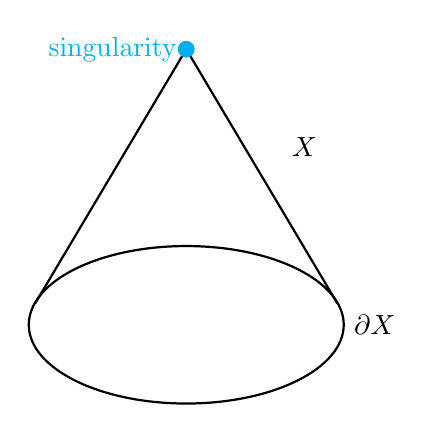
\begin{tikzpicture}
        \draw[thick] (0,0) -- (-1.92,-3.23);
        \draw[thick] (0,0) --  (1.92,-3.23) (1.5,-1.5) node[above]{$X$};
        \draw[thick] (0,-3.5) ellipse (2 and 1)  (2,-3.5) node[right]{$\partial X$};
        \filldraw[cyan] (0,0) circle (.1) (0,0) node[left]{singularity} ;
    \end{tikzpicture}
\end{center}

例如，若 $X$ 局部地是一组方程
\be  f_1(x_1,\dots ,x_n) = f_2(x_1,\dots ,x_n) = \dots =f_k(x_1,\dots ,x_n) =0\subset \bbR[x_1,\dots , x_n] \ee
的交集，则
% ==== 原文 PDF 第 40 页 ====
“边界”$\ptl X$ 由子空间
\be  f_1 = f_2 =\dots =f_k = \sum_{i=1}^n x_i^2 -\varepsilon^2 = 0  \ee
给出，它构成半径为 $\varepsilon$ 的 $S^{n-1}$。

现设 $\ptl X$ 光滑，且存在非平凡的挠拓扑闭链 $[\alpha]\in H_i(\ptl X,\bbZ)$，其挠阶为 $l$，使得 $l[\alpha]=0$。可以构造一个子锥 $\Sigma_{i+1}[\alpha]\subset X$，即 $[\alpha]$ 上的锥，如图~\ref{fig:cones} 所示。于是可以把高形式对称性下的带荷对象构造为绕 $\Sigma_{i+1}[\alpha]$ 缠绕的 M2 或 M5 膜\footnote{确切地说，$\Sigma_{i+1}[\alpha]\in \frac{H_{i+1}(X,\ptl X,\mb{Z})}{H_{i+1}(X,\mb{Z})}$，其中 $H_{i+1}(X,\ptl X,\mb{Z})$ 是 $(X,\ptl X)$ 的相对同调群。}，具体地说，

\begin{enumerate}
    \item 绕 $\Sigma_{i+1}[\alpha]$ 的 M2 膜在 $\bbZ_l^{(2-i)}$ 下带荷，即电的 $(2-i)$-形式对称性。
    \item 绕 $\Sigma_{i+1}[\alpha]$ 的 M5 膜在 $\bbZ_l^{(5-i)}$ 下带荷，即磁的 $(5-i)$-形式对称性。
\end{enumerate}

\begin{yizhu}
指数 $2-i$ 与 $5-i$ 来自维数计数，并非任取：锥 $\Sigma_{i+1}[\alpha]$ 的实维数为 $i+1$，M2 膜的世界体积为 3 维，绕锥缠绕后在 $\bbR^{d-1,1}$ 中留下的对象维数为 $3-(i+1)=2-i$；M5 膜的世界体积为 6 维，相应为 $6-(i+1)=5-i$。按本讲义的约定，$q$-形式对称性作用于 $q$ 维对象，故 M2、M5 分别给出电、磁两种对称性的带荷对象（M2 电耦合于 $C_3$，M5 磁耦合于对偶的 $C_6$）。更须注意 $[\alpha]$ 是挠闭链而非普通闭链：$\Sigma_{i+1}[\alpha]$ 是相对同调中的“锥”，其边界为 $[\alpha]$（脚注 9 用相对同调群把这一点说清楚），而 $l[\alpha]=0$ 正是群为 $\bbZ_l$ 而非 $\bbZ$ 的几何来源。
\end{yizhu}

注意，上述两个对称性由非对易的挠通量生成，且它们彼此并不局域\cite{DelZotto:2015isa,Albertini:2020mdx}。在良定义的（绝对）理论中，需要选择一个极化（polarization），这类似于 $SU(N)$ 规范理论的情形。也就是说，可以保留 M2 膜而得到电的 $(2-i)$-形式对称性，或保留 M5 膜而得到磁的 $(5-i)$-形式对称性。

\begin{yizhu}
“极化”指的是绝对理论中允许哪一族膜作为带荷对象：两族对称性生成元由非对易的挠通量给出、彼此不局域，因而不能在同一个绝对理论中同时存在。这与 $d=4$ 麦克斯韦理论中电、磁 1-形式对称性只能择一的情形同构（电磁对偶把两者互换），也类似 $SU(N)$ 规范理论中威尔逊线与 't Hooft 线的选择：一种选择对应电极化，另一种对应磁极化。选定 M2 后，M5 膜便成为该绝对理论中的非局域拓扑缺陷，反之亦然。原文所引文献中有关于非对易挠通量（non-commutative torsional flux）的专门讨论，可对照阅读。
\end{yizhu}

该机制也适用于 IIA/IIB 弦理论，此时带荷对象是 D$p$-膜而非 M2/M5 膜。

\begin{figure}[htbp]
    \centering
    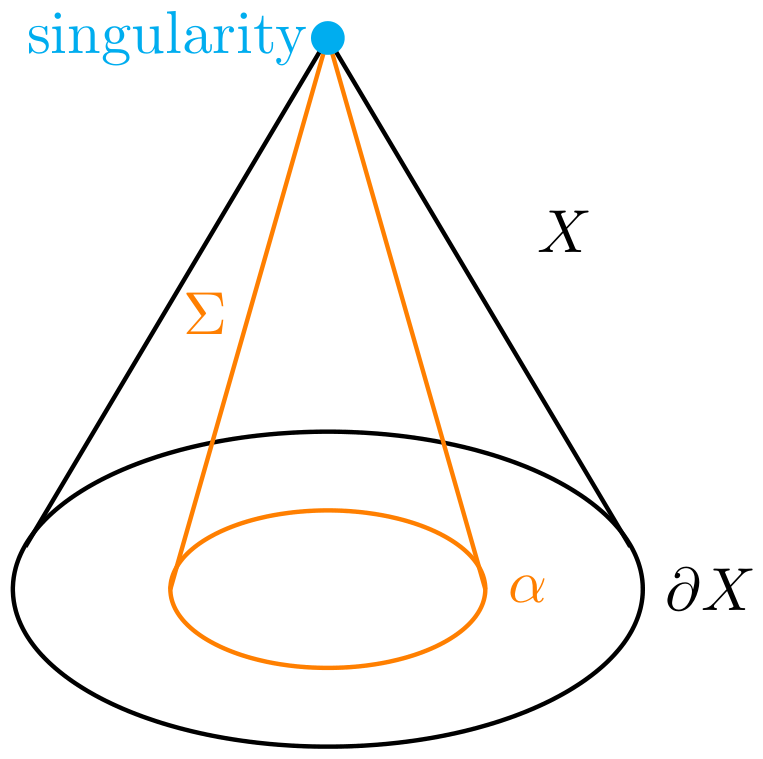
\includegraphics[width=0.30\linewidth]{figures/figure-7.png}
    % [原文图注为空]
    \caption{}
    \label{fig:cones}
\end{figure}

% ==== 原文 PDF 第 41 页 ====
\subsubsection{5 维 $\mathcal{N}=1$ 超共形场论}

在五维，一个重要的特征是：所有（超对称）规范理论在紫外都是强耦合的，例如杨–米尔斯作用量
\be  S_{YM} = \int \dd^5 x \frac{1}{g_{YM}^2} (F_{\mu\nu}F^{\mu\nu}) \ \Rightarrow \ [g_{YM} ] = -\frac{1}{2}  \ee
当能标 $\to\infty$ 时，$g_{YM}$（以该能标为单位）$\to0$，规范理论变得无限强耦合。在一定条件下，超对称规范理论可以紫外完备化为带有 8 个超荷的 $\cN=1$ 超共形场论（SCFT），例如可参见\cite{Seiberg:1996bd,Morrison:1996xf,Intriligator:1997pq,Aharony:1997bh,Benini:2009gi,Kim:2012gu,Bergman:2013aca,Zafrir:2014ywa,Hayashi:2015zka,Xie:2017pfl,Ferlito:2017xdq,Hayashi:2018lyv,Jefferson:2018irk,Bhardwaj:2018vuu,Closset:2018bjz,Cabrera:2018jxt,Apruzzi:2018nre,Bhardwaj:2018yhy,Apruzzi:2019vpe,Apruzzi:2019opn,Apruzzi:2019enx,Apruzzi:2019kgb,Bhardwaj:2019fzv,Bhardwaj:2020gyu,Eckhard:2020jyr,Bhardwaj:2020ruf,BenettiGenolini:2020doj,Bhardwaj:2020avz,Closset:2020scj,Closset:2021lwy,Tian:2021cif,Genolini:2022mpi,DelZotto:2022fnw,Collinucci:2022rii,DeMarco:2022dgh,Bourget:2023wlb}。

若在矢量多重态\footnote{超多重态是超对称代数的一个表示，由自旋不同的粒子组成。对于无质量矢量多重态，其中包含矢量场 $A_\mu$、马约拉纳旋量 $\chi$ 与实标量 $\phi$。} $(A_\mu,\chi,\phi)$ 中，实标量 $\phi$ 获得非零真空期望值（VEV，即 $\expval{\phi}\ne 0$），则这一非零 VEV 把原来的、可能非阿贝尔的规范理论/超共形场论破缺为 $U(1)^r$（$r$ 为原规范群的秩）阿贝尔规范理论，带电物质为超多重态\footnote{超多重态中包含一个马约拉纳旋量 $\psi$ 与两个复标量 $\phi$ 及 $\Tilde{\phi}$。} $(\psi,\phi,\Tilde{\phi})$。

这一点有 M 理论实现，我们在第~\ref{sssect:M-th}~节发展的工具正好用得上。考虑紧化在带有奇异点的 Calabi-Yau 三流形 $X$
\footnote{这里的 3 指复维数，就实维数而言是 6。Calabi-Yau 意味着其典范丛平凡。}
上的 11 维 M 理论。从紫外超共形场论到库仑分支（Coulomb branch）的过程，对应于 crepant 解奇（crepant resolution）\footnote{形式上，crepant 解奇是保持典范除子不变的双有理映射。}，即对奇异点作光滑化，同时保持场论的超对称性。

\begin{center}
    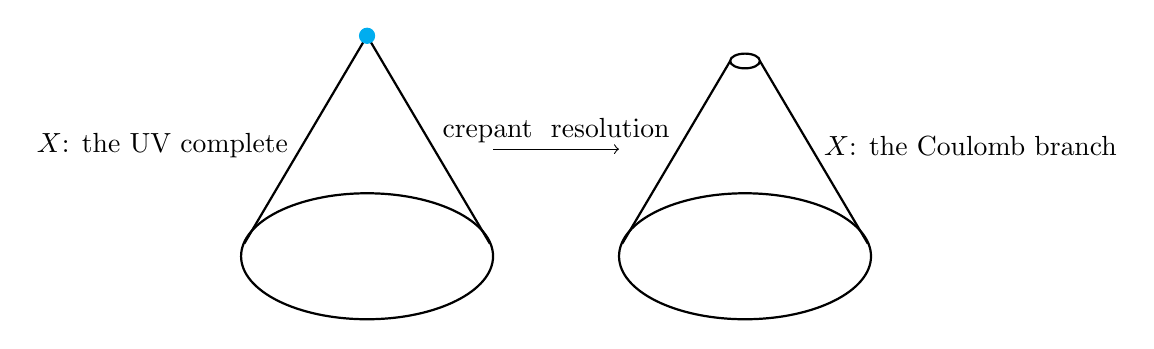
\begin{tikzpicture}[scale = 0.8]
        \draw[thick] (0,0) ellipse (2 and 1);
        \draw[thick] (1.95,0.2) -- (0,3.5)  (-1.95,0.2) -- (0,3.5) ;
        \filldraw[cyan]  (0,3.5) circle (0.12);
        \node at (3,2) { crepant \ resolution};
        \node at (-1.1,1.75) [left] {$X$: the UV complete};
        \node at (7.1,1.75) [right] {$\Tilde{X}$: the Coulomb branch};

        \draw[->] (2,1.7)--(4,1.7);
        \draw[shift = {(6,0)},thick] (0,0) ellipse (2 and 1);
        \draw[shift = {(6,0)},thick] (1.95,0.2)--(0.236,3.1) (-1.95,0.2)--(-0.235,3.1);
        \draw[shift = {(6,0)}, thick] (0,3.1) ellipse (0.236 and 0.117);
    \end{tikzpicture}
\end{center}

在解奇后的 $\Tilde{X}$ 中有紧致 4-闭链 $S_i \ (i\in {1,\cdots ,r})$，每个对应库仑分支上的一个规范群 $U(1)_i$。利用 M 理论 $C_3$ 规范场的展开
\be C_3 = \sum_{r=1}^r A_i \wedge \omega_i  \ee
其中 $\omega_i$ 是 $S_i$ 的庞加莱对偶 2-形式，$A_i$ 是 $U(1)_i$ 规范场。此外还有紧致 2-闭链 $C_j$，绕 $C_j$ 缠绕的 M2 膜给出 $5$ 维中的 BPS 粒子，其
% ==== 原文 PDF 第 42 页 ====
$U(1)_i$ 下的电荷定义为
\be q_{i,j} = {\rm Int}(C_j,S_i)|_{\Tilde{X}}\,,  \ee
即交点数。

\begin{yizhu}[原文疑误]
（4.7）的求和上下限与被加项指标不匹配：原文写作 $\sum_{r=1}^r A_i \wedge \omega_i$，上限用 $r$、被加项却用 $i$，按上下文应为 $\sum_{i=1}^r A_i\wedge\omega_i$（$r$ 为规范群的秩）；此处照原文保留。同段的“$S_i$ 的庞加莱对偶 2-形式”与后文“每个 $s_i$”大小写不一致（后者照原文保留为小写 $s_i$）。此外，源码把集合写成未转义花括号的 $1,\cdots ,r$，排出来是 $i\in 1,\cdots ,r$，应为 $\{1,\cdots ,r\}$，属排版瑕疵，不影响内容。
\end{yizhu}

在一定条件下，可以从 $\Tilde{X}$ 取几何极限。假设每个 $s_i$ 具有 $S^2$-纤维化结构，并取 ${\rm vol}(S^2)\to 0$ 的极限。其图像是：这是非阿贝尔规范理论的极限，因为绕 $S^2$ 的 M2 膜就是 W-玻色子，所以把体积取为零就使相应（关于指标 $i$）的 W-玻色子变为无质量。这与 5 维非阿贝尔规范理论的红外物理描述一致。

作为一个详细的例子，考虑环面（toric）CY3 奇点 $X$ 的情形，它是 Sasaki-Einstein 五维流形\footnote{Sasaki-Einstein 流形 $X$ 定义为度规锥 $\mb{R}_{>0}\times X$ 为 K\"ahler 且 Ricci 平坦的流形\cite{Sparks:2010sn}。对于 $Y^{N,k}$，它可以描述为 $S^2\times S^2$ 上的 $S^1$-丛，其第一陈类 $c_1$ 由 $N$ 与 $k$ 参数化。} $Y^{N,k}$ 上的锥。我们把 $X$ 的 crepant 解奇画成环面图（关于环面 CY3 的记号，例如可参见\cite{Xie:2017pfl,Eckhard:2020jyr}）

\begin{center}
    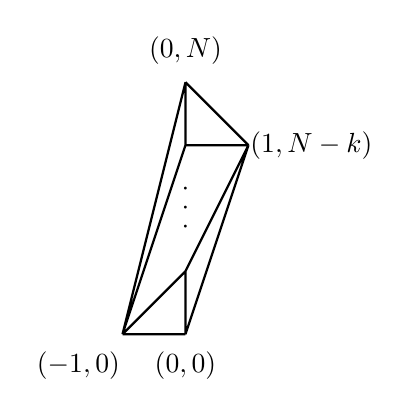
\begin{tikzpicture}[scale = 0.8]
        \draw[thick] (0,1) -- (0,2) (0,1)-- (1,1) (0,2) -- (1,1) (0,2) -- (-1,-2) (0,1) -- (-1,-2) (0,-1) -- (0,-2) (0,-1) -- (1,1) (0,-2) -- (1,1) (0,-1) -- (-1,-2) (0,-2) -- (-1,-2);
        
        \node at (0,2.5) { $(0,N)$};
        \node at (0,-2.5) { $(0,0)$};
        \node at (-1.7,-2.5) { $(-1,0)$};
        \node at (2,1) { $(1,N-k)$};
        \node at (0,0.3) { $\cdot$};
        \node at (0,0) { $\cdot$};
        \node at (0,-0.3) { $\cdot$};
    \end{tikzpicture}
\end{center}

紧致除子 $S_i$（$i=1,\dots,N-1$）都是底为 $S^2$、纤维为 $S^2$ 的纤维化。该理论在红外有非阿贝尔规范理论描述 $SU(N)_k$，其中 $k$ 是陈–西蒙斯能级。

可以用三种不同的方法计算 1-形式对称性，结果彼此相同。这里选择极化，使给定的几何设定具有最大的 1-形式对称性。

\begin{enumerate}
\item{可以计算电荷矩阵 $q_{i,j}$ 的 Smith 标准形（Smith normal form），见 \ref{SmithDecomp}。由 Smith 标准形可读出 1-形式对称性 $\Gamma^{(1)}=\mb{Z}_{\text{gcd}(N,k)}$。}
\item{从链环（link）五维流形 $Y^{N,k}$ 的同调，有
\be
\ba
&H_0(Y^{N,k},\mb{Z})=\mb{Z}\ ,\ H_1(Y^{N,k},\mb{Z})=\mb{Z}_{\text{gcd}(N,k)}\ ,\ H_2(Y^{N,k},\mb{Z})=0\ ,\ \cr
&H_3(Y^{N,k},\mb{Z})=\mb{Z}_{\text{gcd}(N,k)}\ ,\ H_4(Y^{N,k},\mb{Z})=0\ ,\ 
H_5(Y^{N,k},\mb{Z})=\mb{Z}\,.
\ea
\ee
}
\item{从场论论证，$SU(N)$ 的 1-形式中心对称性 $\mb{Z}_N$ 被 5 维陈–西蒙斯项破缺为子群 $\mb{Z}_{\text{gcd}(N,k)}$。}
\end{enumerate}
